\chapter{Modell/ Modellierung des IFE in einem Bandisolators}
\label{sec:model}
%\section{Hameltonien}
Um den inversen Faraday Effekt mit Hilfe der Floquet Theorie in
einem Bandisolator genauer zu untersuchen, wird hier ein mikroskopisches zwei dimensionales Modell
eines Festkörpers mit vier Gitterplätzen herangezogen. Zu Beginn
wird ein System betrachtet, indem sich ein spinloses Elektron aufhält, wobei zwischen dem
zeitunabhängig System, ohne ein elektrisches Feld,
und dem zeitabhängigen System, mit einem in der Zeit periodischen elektrischen Feldes, unterschieden wird.
Darauf folgend wird die Floquet Matrix ??nach dem Abschnitt \ref{sec:matrix}?? für das
zeitabhängige System aufgestellt. Abschließen soll das System für Zwei spinlose Elektronen betrachtet werden.




\section{Zeitunabhängiges System}
Dieses Gittersystem wird durch das Tight-Binding-Modell in zweiter Quantisierung mit periodischen Randbedingungen\cite{czycholl} beschrieben.
Aus diesem ergibt sich der folgende Hamiltonian $H_0$ für das zeitunabhängige System % lautet
\begin{align}
  H_0=\underbrace{J\sum_{i=1}^4 \left(c_{i+1}^\dag c_i^{\phantom{\dag}} + c_{i}^\dag c_{i+1}^{\phantom{\dag}}\right)}_{H_{TB}}
   +\underbrace{\sum_{i=1}^4\left( a_i^{\phantom{\dag}} c_i^\dag c_i^{\phantom{\dag}} \right)}_{H_a}
\end{align}
wobei der Tight-Binding Hamiltonian $H_{TB}$, der Sprünge des Elektron
zwischen den Gitterplätzen beschreibt, durch den Hamilton $H_a$, der die Eigenschaften
eines Bandisolators simuliert, erweitert wird.
Dabei besitzten die Gitterplätz eine lokale ??in dem Vorzeichen ?? alternierende Energie $a$.
Die Gitterplätze sind im Abstand der Gitterkonstante $d$ quadratisch angeordnet
und in der Abbildung \ref{fig:system}
ist eine Skizze des zu untersuchenden Systems dargestellt.


\begin{figure}
   \centering
   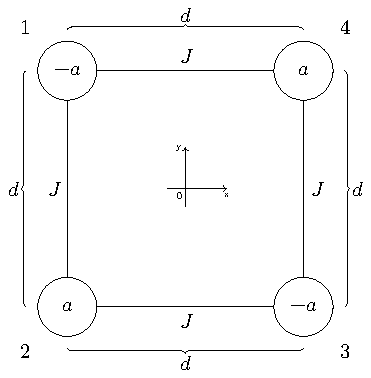
\includegraphics[width=0.5\textwidth]{Programme/Tikz_test/bild_gitter_0.pdf}
   \caption{Skizze des verwendeten 2D-Modell
    des Bandisolators, mit vier Gitterplätzen im Abstand $d$,
   welche die alternierendene lokale Energie $a$ besitzen.
    Elektronen in System können abhängig von dem Tight-Binding-Paramter $J$
   den Gitterplatz wechselen}
   \label{fig:system}
\end{figure}


Durch die Wahl der Basis
\begin{align}
 \ket{1}&=\vec{e}_{1}&    &\ket{2}=\vec{e}_2& &\ket{3}=\vec{e}_3& &\ket{4}=\vec{e}_4,
\intertext{wird über}
H_{ij}&=\braket{i|H|j}
\intertext{die Matrixdarstellung des Hamiltonian}
  H_0&=\begin{pmatrix}
  -a          & \phantom{-}J &\phantom{-}0& \phantom{-}J \\
  \phantom{-}J& \phantom{-}a &\phantom{-}J& \phantom{-}0\\
  \phantom{-}0& \phantom{-}J & -a         & \phantom{-}J \\
  \phantom{-}J& \phantom{-}0&\phantom{-}J & \phantom{-}a
\end{pmatrix}
\end{align}
bestimmt.
Mit Hilfe der stationären Schrödingergleichung
ergeben sich die Eigenwerte
\begin{align}
  E_{1/4}&=\mp\sqrt{a^2+4J^2}&  &E_{2/3}=\mp a
\end{align}
und die Eigenvektoren $\ket{\phi}_n$  des Hamiltonian.

Die Eigenwerte $E_n$ des Hamiltonian sind in der Abbildung \ref{fig:bandstruktur} in einem Niveauschema dargestellte.
\begin{figure}
   \centering
   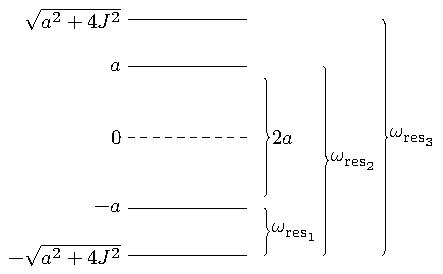
\includegraphics[width=0.6\textwidth]{Programme/Tikz_test/bild_niveau.pdf}
   \caption{Niveauschema für ein Elektron, welches sich in dem System befindent
und die dadurch resultierenden
möglichen Resonanzfrequnzen des Systems.}
   \label{fig:bandstruktur}
\end{figure}

%Ebenfalls kann die für ein Bandisolator charakteristische Bandlücke von $2a$
Die Resonanzfrequenzen des Systems im Grundzustand
\begin{align}
\omega_{\text{res}_1}=\sqrt{a^2+4J^2}-a,
& &\omega_{\text{res}_2}=a+\sqrt{a^2+4J^2},
& &\omega_{\text{res}_3}=2\sqrt{a^2+4J^2} \label{eqn:Resonanz}
\end{align}
werden aus dem Niveauschema \ref{fig:bandstruktur} entnommen. In der Abbildung \ref{fig:bandstruktur} ist ebenfalls die Bandlücke von $2a$
dargestellt.

\section{Zeitabhängiges System}
Als nächstes wird das System durch ein rotierendes E-Feld erweitert, welches
das zirkularpolarisierte Licht simulieren soll, zu sehen in der Abbildung \ref{fig:syst+E}.

\begin{figure}
   \centering
   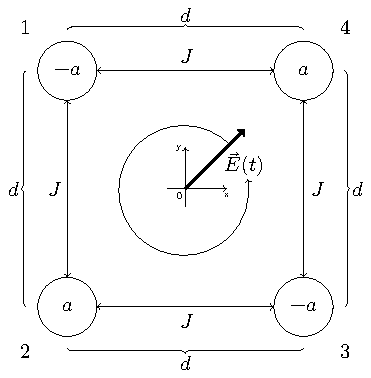
\includegraphics[width=0.5\textwidth]{Programme/Tikz_test/bild_gitter.pdf}
   \caption{Skizze des zeitabhängigen 2D-Modell
wobei zusatzlich zum zeitunabhängigen Modell
ein mit der Zeit rotierendes elektrisches Feld
eingezeicht ist.
  . }
   \label{fig:syst+E}
\end{figure}


Der Hamiltonian wird dafür um den Term
\begin{align}
  H_\text{E-Feld}=\sum_{i=1}^4 \epsilon_i^{\phantom{\dag}} c_i^\dag c_i^{\phantom{\dag}}  \,\,   \quad \quad  \,\, & &\epsilon&=-\vec{E} \vec{r_i}
\end{align}
erweitert. Dabei beschreibt $H_\text{E-Feld}$ die Welchelwirkung zwischen dem elektrischen Feld
\begin{align}
  \vec E=E_0\begin{pmatrix}
\cos\left(\omega t\right)\\
\sin\left(\omega t\right)
 \end{pmatrix},
\end{align}
welches die Amplitude $E_0$, die Frequenz $\omega$ besitzt.
Der Ursprung des Systems wird in den Mittelpunkt des Systems gesetzt.
Somit lauten die Gitterplatz-Vektoren $\vec{r_i}$ in Abhänigigkeit von der Gitterkonstante $d$:
\begin{align}
  \vec{r}_1=\frac{d}{2}\begin{pmatrix}-1  \\ \phantom{-}1 \end{pmatrix},& &
  \vec{r}_2=\frac{d}{2}\begin{pmatrix}-1  \\ -1 \end{pmatrix},& &
  \vec{r}_3=\frac{d}{2}\begin{pmatrix}\phantom{-}1  \\ -1 \end{pmatrix},& &
  \vec{r}_4=\frac{d}{2}\begin{pmatrix}1  \\ 1 \end{pmatrix}.
\end{align}
Der gesamte Hamiltonian des Systems nimmt somit die Form
\begin{align}
%H=J\sum_{i=1}^4 \left(c_{i+1}^\dag c_i^{\phantom{\dag}} + c_{i}^\dag c_{i+1}^{\phantom{\dag}}   +a_i^{\phantom{\dag}} c_i^\dag c_i^{\phantom{\dag}} +\epsilon_i^{\phantom{\dag}} c_i^\dag c_i^{\phantom{\dag}}\right)\\
H=J\sum_{i=1}^4 \left(c_{i+1}^\dag c_i^{\phantom{\dag}} + c_{i}^\dag c_{i+1}^{\phantom{\dag}}\right)
+\sum_{i=1}^4 \left(a_i^{\phantom{\dag}} c_i^\dag c_i^{\phantom{\dag}}\right)
-\sum_{i=1}^4 \left(\vec{E} \vec{r_i}  c_i^\dag c_i^{\phantom{\dag}}\right)
\end{align}
an.


\section{Floquet Matrix des zeitabhängigen Systems}
Für das zeitabhängige System wird wie
in Kapitel \ref{sec:matrix} beschrieben, die
numerische Methode der Floquet Matrix angewendet.
Dafür wird zunächst der Hamiltonian
\begin{align}
H=\underbrace{J\sum_{i=1}^4 \left(c_{i+1}^\dag c_i^{\phantom{\dag}} + c_{i}^\dag c_{i+1}^{\phantom{\dag}}c_i^{\phantom{\dag}}\right)
+ \sum_{i=1}^4\left(a_i^{\phantom{\dag}} c_i^\dag c_i^{\phantom{\dag}}\right)}_{H_0}
-\underbrace{\sum_{i=1}^4\left(\vec{E} \vec{r_i}  c_i^\dag c_i^{\phantom{\dag}}\right)}_{V(t)}
\end{align}
in den zeitunabhänigen Teil $H_0$ und einen in der Zeit periodischen Teil $V(t)$ aufgespalten.
Um die Matrix $\mathcal{H}_\mathrm{F}$ zu berechnen, werden zunächst die Untermatrizen $H^{m-n}$ bestimmt.
Aus der Gleichung \eqref{eqn:H_n_m} folgt
\begin{align}
  H^{m-n}=H_0\delta_{m,n} -\frac{E_0}{2}\left(R_{(-)} \delta_{n+1,m}   +  R_{(+)}\delta_{n-1,m}\right)\\
\end{align}
mit
\begin{align}
  R_{(-)}&=\textbf{diag}\left(
  r_{1_x}-r_{1_y} ;
  r_{2_x}-r_{2_y} ;
  r_{3_x}-r_{3_y} ;
  r_{4_x}-r_{4_y}\right)
\\
  R_{(+)}&= \textbf{diag}\left(
  r_{1_x}+r_{1_y} ;
  r_{2_x}+r_{2_y} ;
  r_{3_x}+r_{3_y} ;
  r_{4_x}+r_{4_y}\right).
\end{align}
Somit ergibt sich die Matrix $\mathcal{H}_F$ nach
der Gleichung \eqref{eqn:H_f} in
Blockschreibweise zu einer Diagonalbandmatrix.
% \begin{align}
%   \mathcal{H}_F=\begin{pmatrix}
%   H^{-n ,-n}+(-n)\hbar\omega  &  H^{-n,-n+1}       &       &    & \\
%   H^{-n+1,-n} &    H^{-n+1,-n+1}+(1-n)\hbar\omega  & \ddots&    & \\
%             &          \ddots                      & \ddots&  \ddots      &    \\
%             &                                      & \ddots&  H^{n-1,n-1}+(n-1)\hbar\omega  & H^{n-1,n}  \\
%             &                                      &       & H^{n,n-1}   & H^{n,n}
% \end{pmatrix}
% \end{align}
Für exakte $\epsilon_{\alpha}$ und $\ket{\Phi_\alpha}$ muss
$N\rightarrow\infty $
, da
dies numerisch jedoch nicht möglich ist, wird
die Matrix $\mathcal{H}_F$ bei einem beliebigen $N$ trunkiert
und somit nur die Fouriermoden bis $N$ in der
Berechnung der QEE und QEZ
berücksichtigt.
Die Matrix $\mathcal{H}_F$ besitzt beispielsweise für eine Trunkierparameter  $N=1$ die Form
\begin{align}
  \mathcal{H}_F=\begin{pmatrix}
  H^{-1,-1}-\mathbb{1}\hbar\omega &  H^{-1,0} &   0 \\
  H^{0,-1}               &  H^{0,0}  &H^{0,1}                  \\
      0                  &  H^{1,0}  & H^{1,1}+\mathbb{1}\hbar\omega
\end{pmatrix}.
\end{align}

\section{Zwei-Elektronen-System}
Dem Modell wird ein Elektron hinzugefügt, in Folge dessen unterliegt das System dem Pauliverbot.
Die Eigenwerte $E_n$ setzen sich dabei aus
linear Kombination der Eigenwerte
des Ein-Elektron-Systems \cite{phillip}
zusammen zu
\begin{align}
E_{1/4}&=\mp\sqrt{a^2+4J^2}-a
&E_{2/6}&=\mp\sqrt{a^2+4J^2}+a
&E_{3/4}&=0
\end{align}.
Somit besitzt das System im Grundzustand die Resonanzfrequenzen
\begin{align}
\omega_{\text{res}_1}&=2a
&\omega_{\text{res}_{2/3}}&=\sqrt{a^2+4J^2}+a \\
\omega_{\text{res}_4}&=2\sqrt{a^2+4J^2}
&\omega_{\text{res}_5}&=2\sqrt{a^2+4J^2}+2a
\end{align}
